\chapter{Relevante Verfahren und Kriterien für die Evaluation}
\label{kriterien}

Die Evaluation der Einsatzmöglichkeiten von ML-Verfahren für das Application Portfolio Management erfolgt in einem festgelegten Kontext. Zunächst soll eine reale Ist-Situation skizziert werden, die während der Bearbeitungszeit vorgefunden wurde.  Auf der Ist-Situation soll die eigentliche Evaluation von Verbesserungsansätzen aufbauen. 

Die ursprüngliche Aufgabenstellung stammte von einem multinationalen Großunternehmen. Wie im Theorieteil beschrieben wurde, werden im Laufe von Softwareentwicklungsprojekten verschiedene Dokumente erstellt (beispielsweise ``System Requirements Specifications`` (SRS), ``Business Requirement Specifications`` (BRS), ``Solution Architecture Statements`` (SAS), ``Detail(ed) Design Specifications`` (DDS)). Diese Dokumente werden normalerweise auf Basis von Standard-Templates angefertigt. Die Dokumente müssen im vorliegenden Szenario manuell ausgewertet werden, um Informationen aus den Dokumenten zu extrahieren oder um Dokumenten-übergreifende Erkenntnisse zu gewinnen. Es wird die These vertreten, dass durch KI- und ML-Ansätze diese manuellen Prozesse unterstützt werden können. Nachfolgend werden zunächst Anwendungsfälle beschrieben und es wird erläutert, mit welchen ML-Verfahren die Anwendungsfälle realisiert werden können. Das Kapitel erläutert außerdem wie und anhand von welchen Kriterien die einzelnen Verfahren evaluiert werden. 

\section{Verfahren zur Ermittlung von Ähnlichkeiten}

%Als Ontologien festgelegt sind im Umfeld der vorliegenden Evaluation beispielsweise die Ontologien ``Architectural Language``, ``Requirements``, ``Design``, ``Logistics``, ``Generic``, die sich jeweils aus verschiedenen Begriffen zusammensetzen, die das Thema der jeweiligen Ontologie beschreiben. Die Begriffe und Begriffspaare können auch gewichtet werden, um zum Ausdruck zu bringen, wie stark der Bezug eines Begriffs wie etwa Capability zu einem Topic wie ARCH ist. Verwendet werden können die Begriffe und die Gewichtungen etwa für eine regelbasierte Themenerkennung. Wenn bestimmte Begriffe einer Ontologie häufig in auszuwertenden Textabschnitten vorkommen, dann erfolgt die Einteilung des entsprechenden Textabschnitts zu einer der festgelegten Ontologien. 

Es wäre für das Application-Portfolio-Management sehr hilfreich, wenn anhand von Text-Dokumenten auf in der Vergangenheit durchgeführte, ähnliche Projekte geschlossen werden kann, um Überschneidungen von Projekten festzuhalten. Der Frage ``Wurde schon einmal versucht, ein bestimmtes Vorhaben umzusetzen`` könnte sich über ein Ähnlichkeitsmaß angenähert werden. Ob das möglich und sinnvoll mit Methoden aus dem Bereich des maschinellen Lernens ist, wird gezeigt in Kapitel 4.1. Es werden zwei Ansätze untersucht.

Die Ermittlung von Ähnlichkeiten ergibt sich durch den Abgleich eines Dokuments mit anderen Dokumenten einer bestehenden Dokumenten-Datenbank. Genutzt werden könnten dazu zum einen regelbasierte Ansätze, aber auch unterschiedliche Vektor-basierte Ansätze, wie sie in Kapitel 2 beschrieben wurden. Damit kann ein Ähnlichkeitsmaß zwischen einzelnen Dokumenten erzeugt werden. Das Ziel ist hier also die Ermittlung der Überschneidung von Projekten, basierend auf dem Inhalt von Dokumenten. So könnten zum Beispiel zwei Projekte identifiziert werden, in denen es um die Entwicklung von Anwendungen mit den gleichen Absichten geht. Vektor-basierte Ansätze, wie sie in Kapitel 2 beschrieben wurden, nutzen Verfahren des maschinellen Lernens und sind daher hier für eine Evaluation von Bedeutung. Regelbasierte Ansätze können in der Praxis sinnvoll sein, sie werden aufgrund des Titels der Arbeit aber nicht näher betrachtet. Weitere Möglichkeiten könnten Nearest-Neighbor-Verfahren bieten, sie wurden jedoch nicht näher evaluiert und werden nur als mögliche Perspektive erwähnt.

\section{Verfahren zur Bestimmung von inhaltlicher Integrität}

Text-Klassifizierungsverfahren (auch: Verfahren zur Topic-Classification) verfolgen das Ziel, einem gegebenen Text eine oder mehrere Klassen zuzuordnen. Ein bekanntes Beispiel ist die Klassifizierung von Emails in die beiden Klassen Spam oder kein Spam. \cite{Gupta} Es wird bei den vorliegenden Dokumenten davon ausgegangen, dass sie viel Text, aber nur wenige echte Informationen enthalten. 
Es werden Ansätze untersucht, mit denen überprüft werden soll, ob Dokumente das beinhalten, was erwartet wird. Ein Kapitel über ``Anforderungen`` sollte idealerweise auch tatsächlich Anforderungen beschreiben.
Dazu kann ein Dokumenten-Template definiert werden, mit erwarteten ``Topics``. Neben einer Klasse ``Requirements`` könnte eine weitere Klasse ``Architectural Language`` heißen. Die Spalte ``Gefundenes Thema`` aus Tabelle \ref{tab:themenerkennung} ist bei diesem Ansatz das durch einen Klassifizierungsansatz zu schätzende Attribut. Voraussetzung für diese Schätzung ist lediglich, dass die Kapitelstruktur der Dokumente sich an die Templates hält. Davon wird in dieser Arbeit ausgegangen. In der Realität kann es durchaus Abweichungen zwischen Template-Kapitelstruktur und Kapitelstruktur der Dokumente geben. Dieses Problem wird hier bewusst ausgeklammert. Nicht gezeigt werden in der Tabelle die eigentlichen Texte, die als Grundlage für die Schätzung verwendet werden. 

\begin{table}[h]
\centering
\begin{tabular}{|l|l|l|l|}
\hline
\textbf{Kapitel} & \textbf{Kapitelüberschrift}                                                           & \textbf{Erwartetes Thema} & \textbf{Gefundenes Thema} \\ \hline
1                & Introduction                                                                          & No special expectation    & ?                         \\ \hline
1.1              & Background                                                                            & No special expectation    & ?                         \\ \hline
1.2              & Purpose of the Document                                                               & No special expectation    & ?                         \\ \hline
2                & System Requirements                                                                   & Requirements              & ?                         \\ \hline
2.1              & \begin{tabular}[c]{@{}l@{}}User Interface and \\ Functional Requirements\end{tabular} & Requirements              & ?                         \\ \hline
2.2              & Technical   Requirements                                                              & Requirements              & ?                         \\ \hline
3                & System Scope                                                                          & Architectural Language    & ?                         \\ \hline
3.1              & Context                                                                               & Architectural Language    & ?                         \\ \hline
3.2              & System Interfaces                                                                     & Architectural Language    & ?                         \\ \hline
3.3              & System Impacts                                                                        & Architectural Language    & ?                         \\ \hline
4                & \begin{tabular}[c]{@{}l@{}}Business Process and \\ Data Definition\end{tabular}       & Architectural Language    & ?                         \\ \hline
4.1              & Business Process Maps                                                                 & Architectural Language    & ?                         \\ \hline
4.2              & High-level Data Model                                                                 & Architectural Language    & ?                         \\ \hline
\end{tabular}

\caption{Ausgangssituation bei der Themenerkennung}
\label{tab:themenerkennung}

\end{table}

Es geht hier letztendlich darum, die inhaltliche Integrität von Dokumenten zu beurteilen, in denen es um die Spezifikationen von Applikationen geht. Dadurch kann die Frage nach der Güte der Dokumentation einer Anwendung bzw. eines Projekts beantwortet werden. Eine Dokumentation mit Inhalten, die besonders stark von ähnlichen historischen Dokumentationen abweicht, könnte identifiziert werden. In Abschnitt 4.2 werden zwei Ansätze zur Schätzung der inhaltlichen Integrität von Texten untersucht.

\section{Verfahren zur automatisierten Erzeugung von Zusammenfassungen}

Es wird hier die These vertreten, dass es ab einer bestimmten Menge von Dokumenten nicht mehr praktikabel ist, manuell alle vorhandenen Dokumentationen zu lesen und zu versuchen, eine Einordnung der Dokumente und damit der Anwendungen vorzunehmen. Eine automatisch generierte Zusammenfassung der Dokumente könnte sinnvoll sein, damit ein verantwortliches Team die Dokumente schneller und effizienter zu- bzw. einordnen kann.

Bei der Erzeugung von Text-Zusammenfassungen kann grundsätzlich unterschieden werden zwischen extraktiven und abstraktiven Algorithmen. Extraktive Algorithmen zur Erzeugung von Textzusammenfassungen entnehmen wichtige Sätze aus Texten, ohne dabei einzelne Wörter oder Formulierungen zu modifizieren \cite[S. 2]{allahyari}. Derartige Ansätze gibt es mindestens seit dem Jahr 1958, als ursprünglich versucht wurde Literaturabstrakte automatisiert zu erzeugen \cite{luhn}. Von den extraktiven Verfahren soll in dieser Arbeit ein Ansatz auf Basis von TF-IDF näher untersucht werden. Nicht untersucht, aber für die Praxis relevant könnte ein Ontologie-basierter Ansatz sein, der die Wichtigkeit von Sätzen berechnet auf Basis der Anzahl bestimmter Signalwörter aus der entsprechenden Ontologie. Signalwörter können dabei zum Beispiel angeben, ob es sich um interessante Sätze, wie Anforderungsbeschreibungen, handelt. Weitere Algorithmen aus der Kategorie der extraktiven Verfahren sind der WordFrequency- sowie der TextRank-Algorithmus. Sie werden nicht näher betrachtet, da davon ausgegangen wird, dass die Güte dieser Verfahren in etwa der des TF-IDF-Ansatzes entspricht. Abstraktive Verfahren hingegen generieren Zusammenfassungen, die neu zusammengestellte Satzkonstellationen enthalten können, die es so in den ursprünglichen Texten gar nicht gegeben hat \cite[S. 258]{Gupta}. Zu den abstraktiven Verfahren die untersucht werden sollen zählt ein vortrainiertes Modell mit dem Namen T5: Text-To-Text Transfer Transformer. 
Die Neuartigkeit und die Geschwindigkeit der Weiterentwicklung dieser Ansätze erlaubt jedoch hier keine ausführliche Untersuchung aller möglichen Verfahren. Indem je ein extraktives und ein abstraktives Verfahren untersucht wird, kann ein grober Vergleich der beiden Ansätze ermöglicht werden. 

Eine Metrik bzw. ein Ansatz zur Bewertung der Qualität von Zusammenfassungen ist ROUGE: A Package for Automatic Evaluation of Summaries, wobei die Abkürzung für Recall Oriented Understudy for Gisting Evaluation steht. ROUGE ist gedacht für den Abgleich von automatisch generierten und von Menschen erstellten Zusammenfassungen. Es gibt von diesem Package verschiedene Implementierungen. Für die Evaluation der Verfahren kann insbesondere Rouge-N in Betracht gezogen werden. Rouge-N erzeugt N-gram Co-Occurence Statistics, beantwortet also etwa die Frage ``wie viele Bi-Gramme aus einer von Menschen erzeugten Zusammenfassung in einer automatisch erzeugten Zusammenfassung vorkommen`` \cite{Lin}. Das mögliche Vorgehen sieht folgendermaßen aus: 
\begin{enumerate}
\item Automatisierte Erzeugung von Zusammenfassungen mit einem der beiden Ansätze
\item Erzeugung einer menschlichen Referenz-Zusammenfassung mit entsprechender Länge
\item Anwendung von Rouge zur Ermittlung der Rouge-Metriken 
\end{enumerate}

Die Güte von Zusammenfassungen wird in dieser Arbeit also mit einer Metrik beurteilt. ROUGE gleicht zwar den Inhalt der Zusammenfassungen ab, kann aber nicht die ``Lesbarkeit`` bewerten, oder ob ein Text aus ``grammatikalischer Sicht sinnvoll ist``. Daher ist die Einschätzung eines Menschen eigentlich immer am aussagekräftigsten. Eine solche Einschätzung ist jedoch nur dann nützlich, wenn die Verfahren überhaupt sinnvolle Ergebnisse produzieren. Wenn in der Realität ausreichend gute Zusammenfassungen mit einem Verfahren erzeugt werden könnten, dann wäre eine Befragung von Projektbeteiligten denkbar, um die Verfahren zu evaluieren. Die Auswertung der Experten-Befragung kann vereinfacht werden durch Verwendung einer standardisierten 5-Punkte LIKERT-Skala (vgl. das Beispiel in Abbildung \ref{Abbildung:Dang}). Eine solche Befragung wurde hier nicht durchgeführt, stattdessen wird ein Vorschlag für eine zukünftige mögliche Befragung gemacht. Die linguistischen Eigenschaften, die untersucht werden, orientieren sich an \cite{Dang}. Sie sind in Abbildung \ref{Abbildung:Dang} in Spalte 1 abgebildet. Es geht um Grammatik, Redundanz-Vermeidung, korrekte Referenzen, sowie darum ob der Fokus auf dem Wesentlichen liegt, und ob Struktur und Zusammenhänge zwischen Sätzen sinnvoll sind. Die Skala reicht von ``sehr unzufrieden`` bis ``sehr zufrieden``. 
 
\begin{figure}[h]
\centering
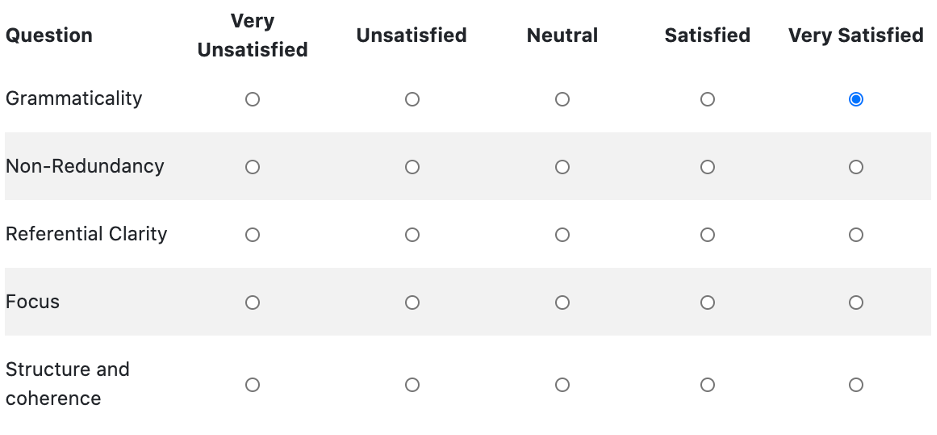
\includegraphics[scale=0.9]{content/pics/Picture_9.png}
\caption{ Potenziell mögliche Befragung, eigener Entwurf in Anlehnung an \cite{Dang}}
\label{Abbildung:Dang}
\end{figure}

In Abschnitt 4.3 werden zwei Verfahren zur Erzeugung von Zusammenfassungen evaluiert.


\section{Verfahren zur automatisierten Schnittstellen-Erkennung}

Dieser Anwendungsfall bezieht sich auf die Erkennung von Schnittstellen (Engl.: Interfaces). Gesucht sind technische Schnittstellen, die Abhängigkeiten zwischen einzelnen Anwendungen darstellen. Das Problem bei der Erkennung einer Schnittstelle anhand von Text in Englischer Sprache ist, dass das Vorkommen des Worts Interface alleine noch nicht unbedingt bedeutet, dass eine technische Schnittstelle identifiziert wurde. Es muss dabei mindestens unterschieden werden zwischen Technischen Schnittstellen (Technical Interfaces, Abk.: TI) und Benutzerschnittstellen (User Interfaces, Abk.: UI). Wenn Schnittstellen automatisch erkannt werden, dann können Sie anschließend visualisiert, etwa wie im Beispiel in Abbildung \ref{Abbildung:Interface_Circle} werden und entsprechend bei Entscheidungen im APM berücksichtigt werden. Das ist der große Mehrwert dieses Ansatzes. Zwei verschiedene Verfahren zur Lösung dieses Anwendungsfalls werden evaluiert in Kapitel 4.4.

\begin{figure}[h]
\centering
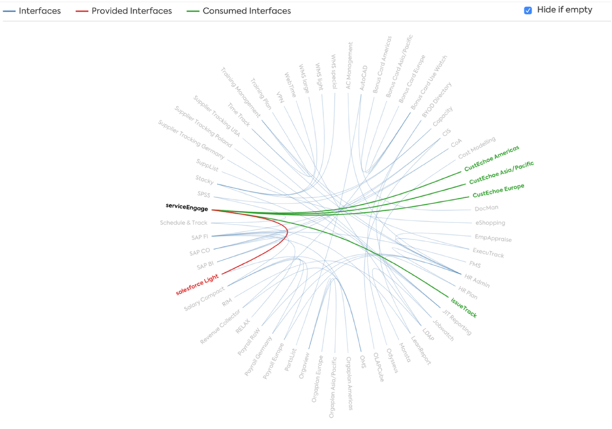
\includegraphics[scale=1.0]{content/pics/Picture_10.png}
\caption{ Schnittstellen-Visualiserung (Interface Circle Map) aus LeanIX, aus \cite{leanix2} }
\label{Abbildung:Interface_Circle}
\end{figure}

Alternativ zu Schnittstellen könnten mit derartigen Verfahren auch beispielsweise Anforderungen als solche klassifiziert werden, d.h. einzelne Sätze würden der Klasse Anforderungen zugeordnet. Sinnvoll im Kontext der IT-Governance ist das Erkennen einer Anforderung innerhalb eines Dokuments dann, wenn es z. B. einen dokumentierten Test für jede Anforderung geben muss. Dann könnte diese Überprüfung auf den durch ML erkannten Anforderungen aufbauen \cite{Vogelsang}. Hier könnte z. B. zwischen funktionalen und nicht-funktionalen Anforderungen unterschieden werden.

Statt den Klassen zur Schnittstellenerkennung könnten also auch andere Klassen verwendet werden. In Kapitel 4.4 erfolgt jedoch eine Begrenzung auf die Schnittstellen-Erkennung.

\section{Zu untersuchende Kriterien}

Einzelne Kennzahlen zur Bewertung von Ergebnissen sind wichtig für die Kommunikation von Ergebnissen an Projektbeteiligte. Hier werden nun Kriterien aufgestellt, anhand derer die Evaluation in dieser Arbeit durchgeführt werden soll. Die Kriterien sind:

\begin{itemize}
  \item Kriterium 1: Einsetzbarkeit der Methode unter den gegebenen Randbedingungen. Für die Evaluation von Verfahren standen bis zu 40 Text-Dokumente (im .docx-Format) zur Verfügung. Es soll überprüft werden, ob die jeweiligen Verfahren mit dieser recht geringen Datenmenge sinnvoll nutzbar sind und einen Mehrwert für das APM erbringen können. Wo es sinnvoll ist, können Metriken wie Accuracy, Precision, Recall, und die F1-Metrik eingesetzt werden.
  \item Kriterium 2: Generelle Einsetzbarkeit im APM-Kontext, unter der Annahme einer beliebig großen Datenmenge. Auch hier können entsprechende Metriken eingesetzt werden. 
  \item Kriterium 3: Vertretbarer Rechenaufwand der Methode. Untersucht werden hier z. B. die Dauer für das Training von Modellen, die Dauer zur Ausführung von Schätzungen, etc.
  \item 
Kriterium 4: Anfallende Kosten, welche zum Beispiel durch notwendige Lizenzierung von Modellen entstehen. Kosten können in der Praxis auch entstehen für das Zusammenstellen und Auszeichnen von Trainingsdaten, was durch Menschen geschehen muss. Es könnte auch sein, dass bei Einsatz gewisser Methoden oder bei Nutzung von großen Modellen eine bestimmte Hardware vorausgesetzt wird. 
\end{itemize}


